%!TEX TS-program = pdflatex
%!TEX TS-options = -shell-escape
% Author: Phil Steinhorst, p.st@wwu.de
% https://github.com/phist91/latex-templates

\newcommand{\obenlinks}{Recurrent and Generative Artificial Neural Networks}
% Author: Phil Steinhorst, p.st@wwu.de
% https://github.com/phist91/latex-templates

\documentclass[%
	paper=a4,
	fontsize=10pt,
	english
	]{scrartcl}

% Basics für Codierung und Sprache
% ===========================================================
	\usepackage{scrtime}
	\usepackage{etex}
	\usepackage{shellesc}					% Compiler-Option -shell-escape benutzen!
	\usepackage[final]{graphicx}			% Einbindung von Grafiken
	\usepackage[utf8]{inputenc}				% Dateien sind UTF8-codiert
	\usepackage{babel}						% deutsche Silbentrennung, etc.
	\usepackage[]{csquotes}	% deutsche Anführungszeichen mit \enquote{...}
% ===========================================================

% Fonts und Typographie
% ===========================================================
	\usepackage{sourcecodepro}
	\usepackage[default]{sourcesanspro}
	\usepackage{nimbusmononarrow}
	
	\usepackage[babel=true,final,tracking=smallcaps]{microtype}
	\DisableLigatures{encoding = T1, family = tt* } % keine Ligaturen für Monospace-Fonts
	\usepackage{ellipsis}
% ===========================================================

% Farben
% ===========================================================
	\usepackage[usenames,x11names,final]{xcolor}
% ===========================================================

% Mathe-Pakete und -Einstellungen
% ===========================================================
	\usepackage{mathtools}					% Tools zum Setzen von Formeln
	\usepackage{amssymb}					% übliche Mathe-Symbole
	\usepackage[bigdelims]{newtxmath}		% moderne Mathe-Font
	\allowdisplaybreaks						% seitenübergreifende Rechnungen
	\usepackage{bm}							% math bold font
	\usepackage{bbm}
	\usepackage{wasysym}					% noch mehr Symbole
% ===========================================================

% TikZ
% ===========================================================
	\usepackage{tikz}
	\usepackage{tikz-cd}					% kommutative Diagramme
	\usetikzlibrary{arrows.meta}			% mehr Pfeile!
	\usetikzlibrary{calc}					% TikZ kann rechnen
	\tikzset{>=Latex}						% Standard-Pfeilspitze
% ===========================================================

% Seitenlayout, Kopf-/Fußzeile
% ===========================================================
	\usepackage{scrpage2}
	\pagestyle{scrheadings}
	\usepackage[top=3cm, bottom=3cm, left=2.5cm, right=2cm]{geometry}
	\clearscrheadfoot 
	\setheadsepline{0.4pt}			 					% Linie in Kopfzeile
	\setfootsepline{0.4pt}								% Linie in Fußzeile
	\setkomafont{pagehead}{\bfseries}					% Schriftart Kopfzeile
	\setkomafont{pagefoot}{\normalfont\footnotesize}	% Schriftart Fußzeile 
	\cfoot{\thepage}									% Seitenzahl unten Mitte
	\lohead{\obenlinks}	% Titel oben links
	\raggedbottom							% Flattersatz
	\usepackage{setspace}					% erweiterte Abstandsoptionen
	\onehalfspacing							% Zeilenabstand 1.5-fach
	\setlength{\parindent}{0pt}				% Einrückung neuer Absätze
	\setlength{\parskip}{0.5\baselineskip}	% Abstand neuer Absätze
% ===========================================================

% Hyperref für Referenzen und Hyperlinks
% ===========================================================
	\usepackage[%
		hidelinks,
		pdfpagelabels,
		bookmarksopen=true,
		bookmarksnumbered=true,
		linkcolor=black,
		urlcolor=SkyBlue2,
		plainpages=false,
		pagebackref,
		citecolor=black,
		hypertexnames=true,
		pdfborderstyle={/S/U},
		linkbordercolor=SkyBlue2,
		colorlinks=false,
		backref=false]{hyperref}
	\hypersetup{final}
% ===========================================================

% Listen und Tabellen
% ===========================================================
	\usepackage{multicol}
	\usepackage[shortlabels]{enumitem}
	\setlist{itemsep=0pt}
	\setlist[enumerate]{font=\sffamily\bfseries}
	\setlist[itemize]{label=$\triangleright$}
	\usepackage{tabularx}
% ===========================================================

% minted
% ===========================================================
\usepackage{minted}
\setminted{%
	style=default,
	fontsize=\small,
	breaklines,
	breakanywhere=false,
	breakbytoken=false,
	breakbytokenanywhere=false,
	breakafter={.,},
	autogobble,
	numbersep=3mm,
	tabsize=4,
	linenos,
	frame=lines
}
\setmintedinline{%
	fontsize=\normalsize,
	numbers=none,
	numbersep=12pt,
	tabsize=4,
}

% Weitere Importe
% ===========================================================
\usepackage{todonotes}
% ===========================================================


%%%%%%%%%%%%%%%%%%%%%%%%%%%%%%%%%%%%%%%%%%%%%%%%%%%%%%%%%%%
%%% Ab hier folgen nur noch vordefinierte Mathe-Befehle %%%
%%%%%%%%%%%%%%%%%%%%%%%%%%%%%%%%%%%%%%%%%%%%%%%%%%%%%%%%%%%

\newcommand{\BB}{\mathbb{B}}
\newcommand{\CC}{\mathbb{C}}
\newcommand{\NN}{\mathbb{N}}
\newcommand{\QQ}{\mathbb{Q}}
\newcommand{\RR}{\mathbb{R}}
\newcommand{\ZZ}{\mathbb{Z}}
\newcommand{\oh}{\mathcal{O}}						
\newcommand{\ol}[1]{\overline{#1}}
\newcommand{\wt}[1]{\widetilde{#1}}
\newcommand{\wh}[1]{\widehat{#1}}

\DeclareMathOperator{\id}{id} 				% Identität
\DeclareMathOperator{\pot}{\mathcal{P}}		% Potenzmenge

% Klammerungen und ähnliches
\DeclarePairedDelimiter{\absolut}{\lvert}{\rvert}		% Betrag
\DeclarePairedDelimiter{\ceiling}{\lceil}{\rceil}		% aufrunden
\DeclarePairedDelimiter{\Floor}{\lfloor}{\rfloor}		% aufrunden
\DeclarePairedDelimiter{\Norm}{\lVert}{\rVert}			% Norm
\DeclarePairedDelimiter{\sprod}{\langle}{\rangle}		% spitze Klammern
\DeclarePairedDelimiter{\enbrace}{(}{)}					% runde Klammern
\DeclarePairedDelimiter{\benbrace}{\lbrack}{\rbrack}	% eckige Klammern
\DeclarePairedDelimiter{\penbrace}{\{}{\}}				% geschweifte Klammern
\newcommand{\Underbrace}[2]{{\underbrace{#1}_{#2}}} 	% bessere Unterklammerungen
% Kurzschreibweisen für Faule und Code-Vervollständigung
\newcommand{\abs}[1]{\absolut*{#1}}
\newcommand{\ceil}[1]{\ceiling*{#1}}
\newcommand{\flo}[1]{\Floor*{#1}}
\newcommand{\no}[1]{\Norm*{#1}}
\newcommand{\sk}[1]{\sprod*{#1}}
\newcommand{\enb}[1]{\enbrace*{#1}}
\newcommand{\penb}[1]{\penbrace*{#1}}
\newcommand{\benb}[1]{\benbrace*{#1}}
\newcommand{\stack}[2]{\makebox[1cm][c]{$\stackrel{#1}{#2}$}}	% Präambel (ohne die geht nichts!)
\begin{document}
\begin{center}
	\begin{tabular}{|rlp{4cm}rl|}
	\hline
	 \textbf{Exercise Sheet} & 04  &  & \textbf{1. Team Partner:} & Lennart Slusny  \\
	 \textbf{Task} & 01 & & \textbf{2. Team Partner:} & Joschka Strüber \\ \hline
	\end{tabular}
\end{center} 

Based on the Differential Evolution Example, we implemented an echo state network with differential evolution. The model is implemented using a three-layer recurrent neural network for three inputs, a small reservoir and three outputs for the three-dimensional coordinates of the target.  

%-ein bisschen mehr beschreiben was wir gemacht haben
For training, we collected a data set of about 2400 consecutive data points. Surprisingly, the model is fairly stable for a wide variety of hyper parameters. Using a smaller reservoir of 30 or less neurons also works, but it requires a larger amount of training steps. The same appears to be even more true, if using a smaller training set. While the cost of each iteration is lower, the amount of steps to reach good results, is much higher. 

If the training set is too short, the RMSE also increases significantly and we recommend to use at least 1000 training points. For example, using 500 instead of 1600 training steps for our final parameters, increases the RMSE by one order of magnitude. In practice, this model still performs good and there is no visual difference compared to the one performing better on paper. 

One of the most interesting parameters is the feedback scaling that greatly decreases the learned output weights. We were able to get good results for any values between $10^{-8}$ and $10^{-12}$. If we increased it too much, e.g. $10^{-7}$, we were still able to get good RMSE values on the test set, but for some reason the predicted trajectories were both wrong and unstable.

When the hyper parameters are chosen sensibly, the neural evolution algorithm finds a working set of weights very quickly, often getting solid results in ten iterations or less. Usually, a few hundred training iterations are more than enough to reach very good results. Training for much longer (500, 1000 or 10,000 iterations) has diminishing returns and the chance to find a very slightly better model decreases quickly.

Our final model was trained using 300 washout steps, 1600 for training and 400 for testing. The reservoir size is 50 and the feedback scaling $10^{-9}$. 1000 optimization steps were used, but 100 probably would have been sufficient as well. The model reaches an RMSE of about $3\cdot 10^{-4}$ on the test set. 

\begin{figure}[b]
	\centering
	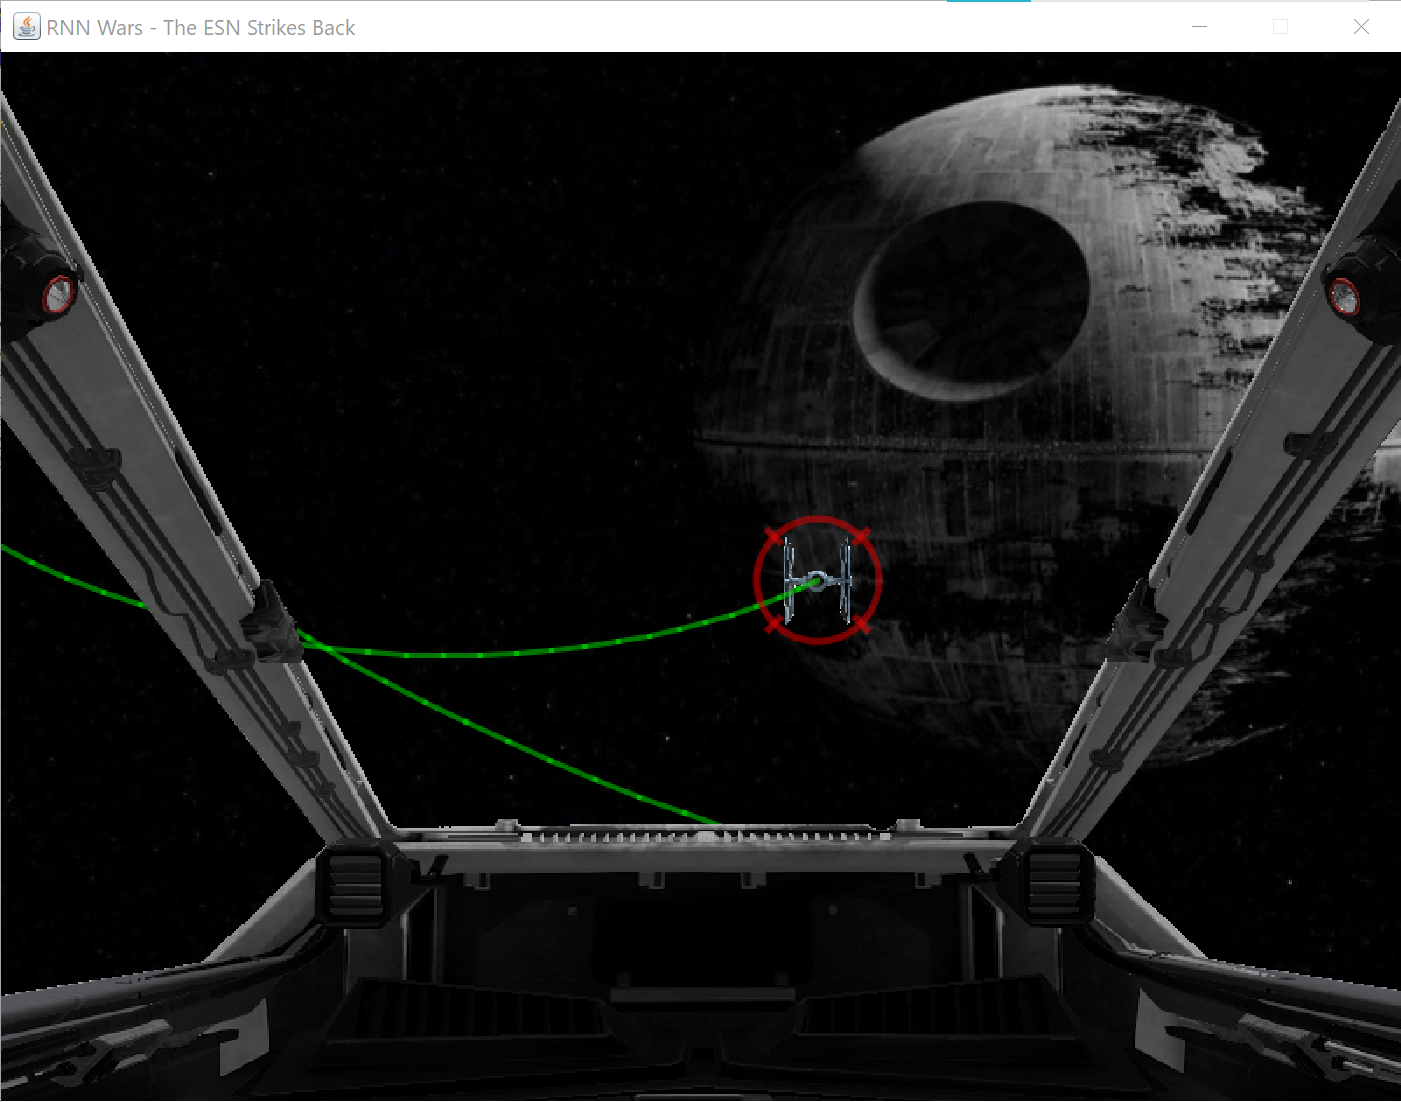
\includegraphics[width=0.475\linewidth]{washout}%
	\hfill
	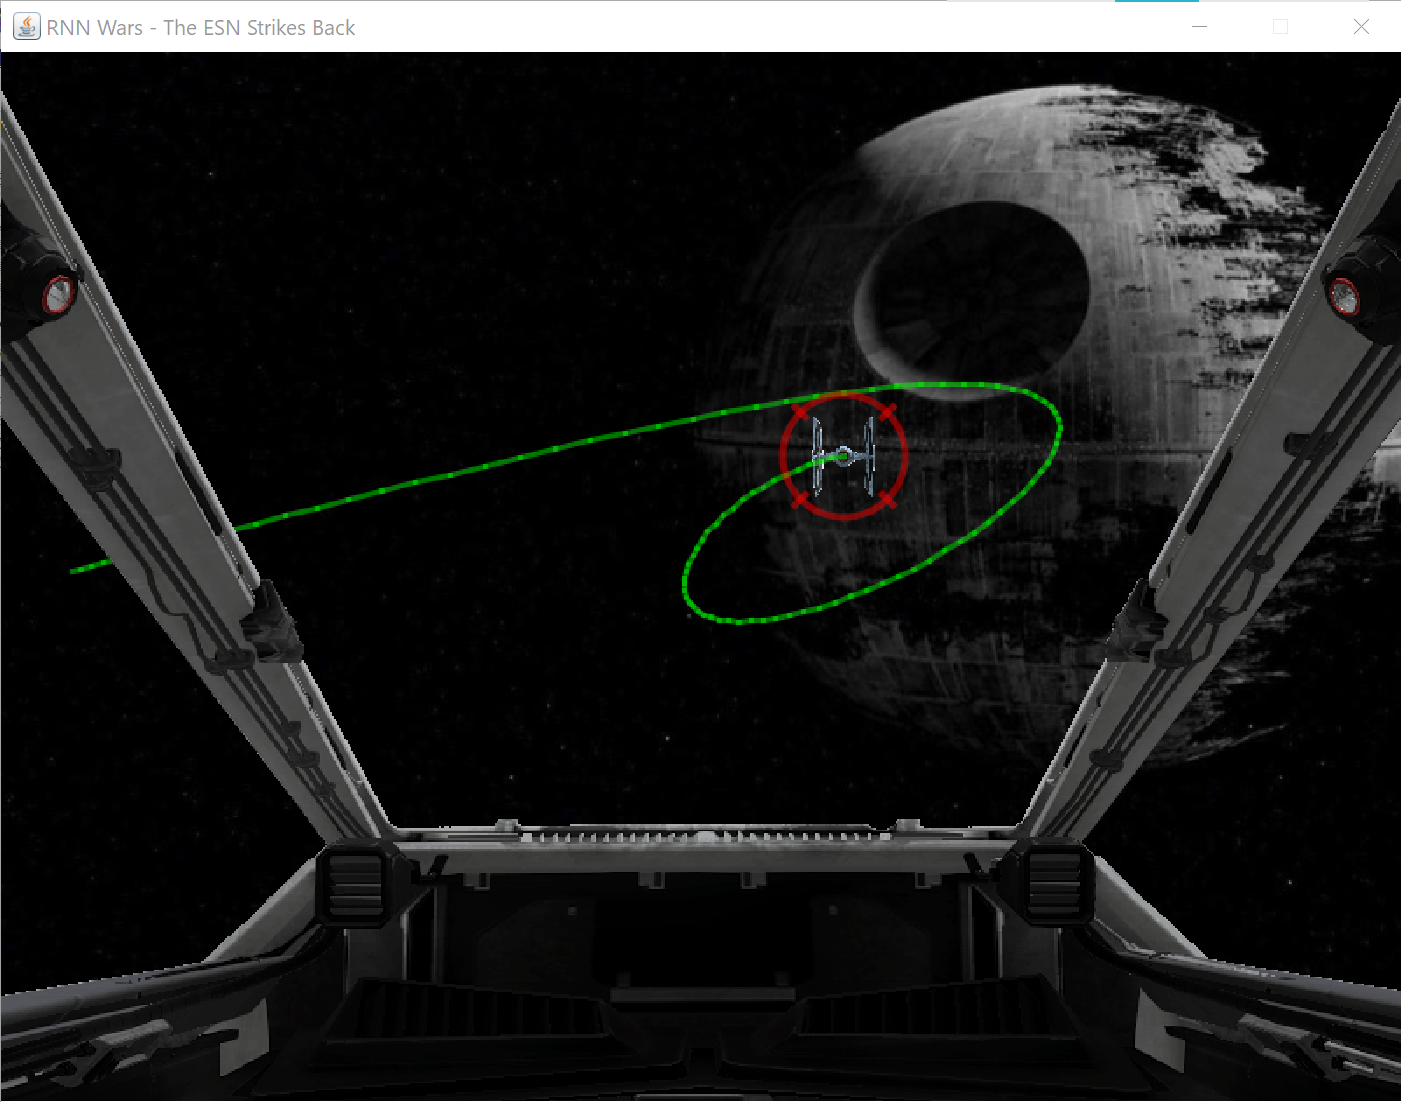
\includegraphics[width=0.475\linewidth]{trajectory}
	\caption{The expected trajectories during and after washout.}
	\label{img:trajectory}
\end{figure}

%-Datensatz erklären
%-Verhalten bei verschiedenen Hyperparametern, Datensätzen, ...
%-unsere finalen Hyperparameter

The trajectory projection simply uses a copy of the pretrained model and computes the next 100 predicted time steps as absolute coordinates. Taking a copy instead of the original network is important, because by computing 100 forward passes, we change the model's activations. Continuing with those activations at the next simulation step, would return the wrong results, because the model expects to be 100 time steps in advance. For this reason, we copy the activations of the model to the copy, which is used for the projection.

After locking on the target, the trajectory starts to be unstable in the beginning. This is to be expected, because we are essentially in the washout stage of the ESN. This can be seen in Figure \ref{img:trajectory} on the left. After a few hundred time steps, the predictions stabilize and remain basically unchanged after each simulation step, as seen on the right. 

Based on visual confirmation, the predicted trajectories are very good and the TIE fighter is at the expected position at each time step. The provided RNN to steer the missiles is not perfect, but we are able to hit the space ship in about 90 to 95\% of cases.


\end{document}